\documentclass[12pt]{article}

\usepackage{styles/sbc-template}
\usepackage[brazil]{babel}   
\usepackage[utf8]{inputenc}
\usepackage{graphicx}

\begin{document}
	\section*{Introdução}
	ESG é a sigla para Environmental, Social and Governance (Ambiental, Social e Governança), e se refere a um conjunto de práticase princípios que as empresas podem adotar para demonstrar seu compromisso com a sustentabilidade e a responsabilidade social. Seus pilares são caracterizados da seguinte forma:
	\begin{itemize}
		\item Ambiental: como a empresa se relaciona com o meio ambiente, abrangendo questões como utilização de recursos naturais, emissão de poluentes e impactos ambientais em geral.
		\item Social: como a empresa se relaciona com seus funcionários, clientes e a comunidade onde está inserida, e abrange questões como diversidade, inclusão e bem-estar dos envolvidos.
		\item Governança: se refere à forma como a empresa é administrada, e abrange questões como a transparência e ética corporativa, assim como a sua estruturação hierárquica.
	\end{itemize}
	Nos últimos anos, o ESG vem ganhando força devido ao aumento da conscientização sobre a sustentabilidade e da responsabilidade social das empresas, algo que impacta inclusive a decisão de investidores para uma melhor alocação de capital.
	
	É possível observar que empresas que adotam o ESG possuem uma boa reputação perante o público, e tais iniciativas podem ser um indicativo da saúde corporativa da empresa, já que exigem planejamento e execução bem estruturados para serem realizados.
	
	Embora não existam legislações sobre o ESG, as normas preexistentes podem guiar a adoção dessas práticas para as empresas, tendo em vista que tangem assuntos semelhantes. Um exemplo disso é o Sistema de Gestão Ambiental da ISO 14000, um conjunto de regras que estabelece, um \emph{framework} para que as empresas gerenciem seu impacto ambiental, algo de extrema importância no pilar ambiental do ESG.
	
	Em paralelo a isso, a ONU estabeleceu 17 objetivos para serem alcançados pelos países até 2030 (Objetivos de Desenvolvimento Sustentável – ODS). Muitos destes objetivos estão em alinhamento com o ESG, pois buscam o progresso de forma sustentável e socialmente justa.
	
	O ESG, por ser um conceito bastante abrangente, pode ser implementado em qualquer setor da economia, o que não deixa de fora as atividades econômicas mais recentes. Portanto, empresas de tecnologia, que já possuem inovação e questões sociais atuais em pauta, são alguns dos setores com mais facilidade de adotar tais práticas.
	Estudo de caso: empresas de tecnologia e provedores de serviços de nuvem
	
	\section*{Estudo de caso: ESG em empresas de tecnologia e infraestrutura em nuvem}
	
	Considerando um crescimento de 15\%, metade do ritmo dos últimos cinco anos, os ativos de ESG sob gestão poderiam subir para mais de um terço do total global projetado de US\$ 140,5 trilhões até 2025. Os ativos de ESG estão no caminho para alcançar US\$ 53 trilhões, com base em nossa análise, um aumento em relação aos US\$ 37,8 trilhões registrados até o final do ano. Eles saltaram de US\$ 30,6 trilhões em 2018 para US\$ 22,8 trilhões em 2016 \cite{bloombergprofessionalservicesESGAssetsMay2021}
	
	Uma pesquisa recente da Harris realizada em nome do Google Cloud indica que apenas 22\% das organizações têm um programa oficial de ESG em vigor e estão mensurando seu impacto, uma queda de 3\% em relação ao ano anterior. Isso coloca os executivos em uma posição desconfortável quando se trata de suas declarações públicas, com 87\% dos entrevistados afirmando que desejam que suas organizações tenham melhores ferramentas para medir os esforços de sustentabilidade, a fim de estabelecer metas mais precisas \cite{googlecloudUnderstandingHowYour2023}.
	
	Um estudo da consultoria KPMG apontou que 76\% das empresas brasileiras já incluem iniciativas ESG em suas estratégias de negócio. Este estudo avaliou as práticas ambientais, sociais e de governança corporativa de 200 das maiores empresas listadas na B3, a bolsa de valores brasileira sediada em São Paulo \cite{deKPMGESGYearbook2023}.
	
	Das empresas avaliadas, é possível observar que o setor de papel e celulose manteve o maior score ESG em todos os anos analisados, enquanto \emph{utilities} foi o setor que mais evoluiu no período de 2018 a 2022.
	

	
	Embora correlação não implique causalidade, as empresas com melhores avaliações de ESG tem um maior valor de mercado e melhores retornos financeiros. Além disso, empresas que adotam medidas sustentáveis tem mais chances de conquistar a preferência do consumidor, uma vez que os aspectos abordados pelas iniciativas visam melhorar o ambiente como um todo, afetando os envolvidos direta e indiretamente com o negócio \cite{cabralPraticasESGAplicadas2023}.
	
	
	Os ativos globais ESG estão a caminho de ultrapassar os 53 bilhões de dólares até 2025, representando mais de um terço dos 140,5 biliões de dólares em ativos totais sob gestão projetados. Uma tempestade perfeita criada pela pandemia e pela recuperação verde nos EUA, na UE e na China provavelmente revelará como o ESG pode ajudar a avaliar um novo conjunto de riscos financeiros e a aproveitar os mercados de capitais. A representação desse constante crescimento pode ser observada na Figura \ref{fig:projections}.
	
	\begin{figure}[h]
		\centering
		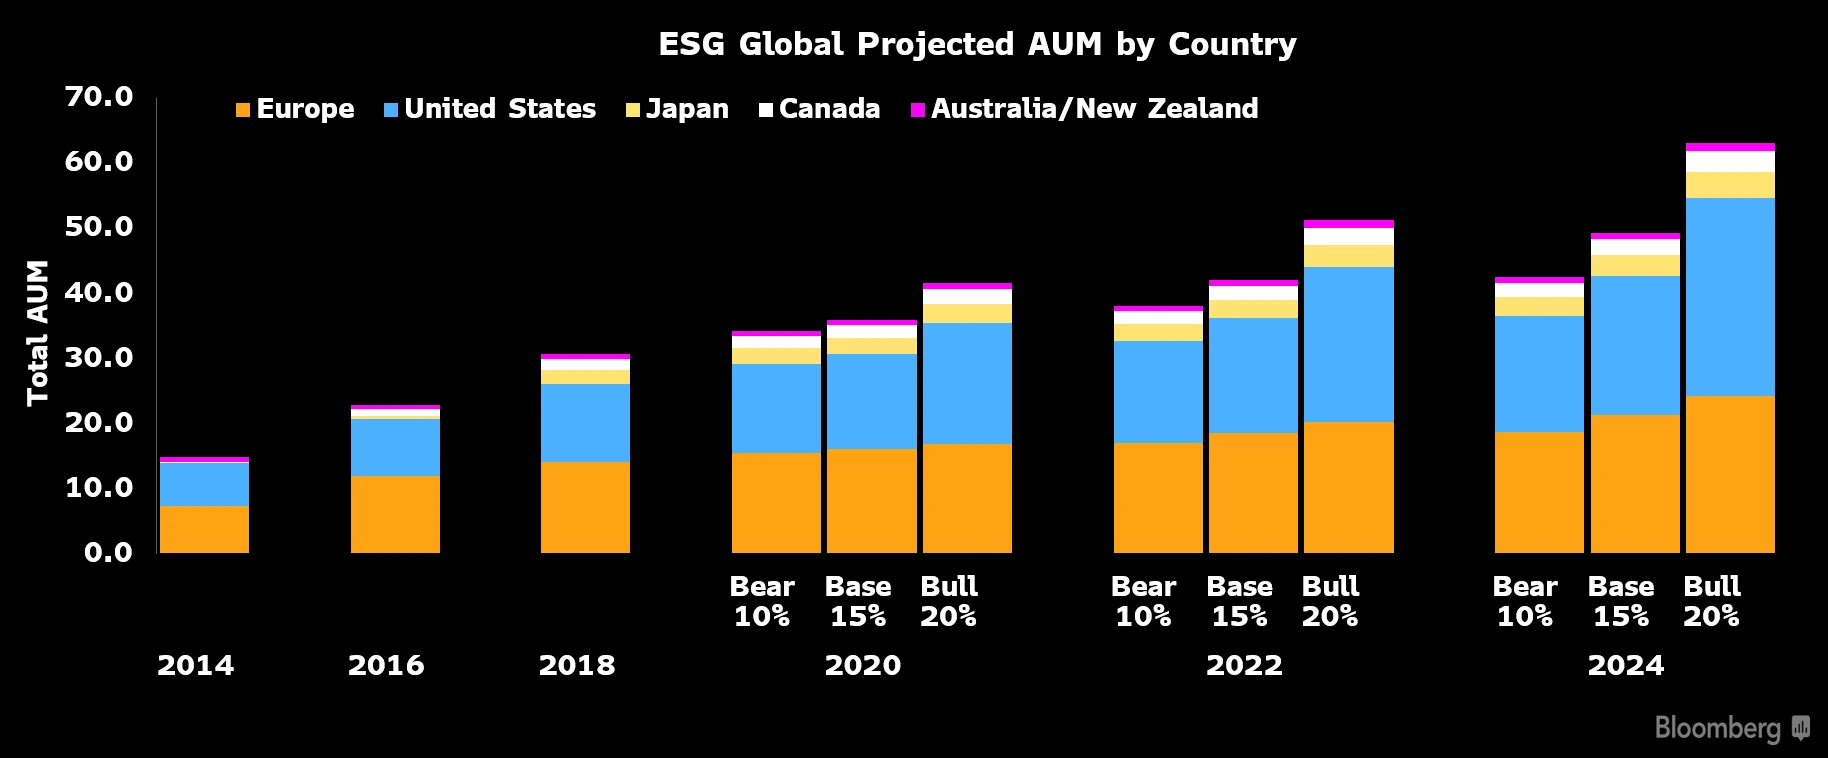
\includegraphics[scale=0.2]{pictures/esg-projections.png}
		\caption{Histórico e projeções do ESG}
		\label{fig:projections}
	\end{figure}
	
	\subsection*{ESG no setor de tecnologia}
	
	O ESG está entre as prioridades das empresas de tecnologia. A constatação é de um levantamento da empresa Schneider Electric. O estudo foi feito por meio do desdobramento de três pesquisas com foco em sustentabilidade em operações de Tecnologia da Informação (TI) desenvolvidos por 451 Research, S\&P Market Intelligence e Forrester Consulting juntamente com Canalys \cite{paceteESGPrioridadePara2022}.
	
	A pesquisa da Canalys determinou que os parceiros de canal de TI estão investindo em estratégias de sustentabilidade, mas lutam para traduzir o investimento em ação e, por isso, não possuem uma resposta clara sobre como atingir tal objetivo. Com 61\% com pessoal dedicado à sustentabilidade, apenas um terço estabeleceu metas ESG \cite{paceteESGPrioridadePara2022}.
	
	O documento da Forrester Consulting descobriu que, para 73\% dos entrevistados, a sustentabilidade é a segunda prioridade geral, mas apenas 33\% dizem que suas organizações criaram um plano estratégico de sustentabilidade \cite{paceteESGPrioridadePara2022}.
	
	O documento da 451 Research revelou que as organizações empresariais acreditam que seus programas de sustentabilidade são mais avançados do que realmente são, pois “as avaliações de maturidade de quase metade (48\%) dos entrevistados não corresponderam a uma resposta anterior” \cite{paceteESGPrioridadePara2022}.
	
	\subsection*{Como a tecnologia auxilia no ESG}
	
	Quando se trata do avanço tecnológico, muitas das inovações dos últimos anos contribuem para um melhor uso dos recursos naturais, assim como reduzir os impactos das atividades econômicas no ambiente. Não apenas isso, mas também melhorias socioeconômicas locais e de processos internos para alcançar os objetivos do ESG \cite{cabralPraticasESGAplicadas2023}.
	
	Alguns exemplos são:
	
	\begin{itemize}
		\item a redução do consumo de energia e emissões de gases de efeito estufa;
		\item inclusão social e o acesso à educação, saúde, cultura e informação, por meio de plataformas digitais, aplicativos, dispositivos móveis, redes sociais, entre outras;
		\item melhoria da governança corporativa e a transparência, por meio de ferramentas de gestão, auditoria, \emph{compliance}, segurança da informação, \emph{blockchain}, entre outras;
	\end{itemize}
	
	\subsection*{Como o ESG pode ser implementado em empresas de tecnologia}
	
	
	
	\bibliographystyle{styles/sbc}
	\bibliography{references}
\end{document}

